\section{Omliggende Implementation}
% motivation for creating this theme

\begin{frame}{Omliggende Implementation}
	Omliggende Implementation
	\begin{itemize}
    \item<2-> DWPopulator
    \item<3-> Intermediate Representation
  \end{itemize}
\end{frame}

\subsection{DWPopulator}
\begin{frame}{DWPopulator}{}
  Hvornår bruges den?
  \begin{itemize}
    \item<1-> Populate test-database
    \item<2-> Bruger pygrametl program
    \item<3-> Udskiftning af sources
  \end{itemize}
\end{frame}

\begin{frame}{DWPopulator}{}
	Hvorfor nyttig?
  \begin{itemize}
		\item<1-> Source-to-target
		\item<2->[] 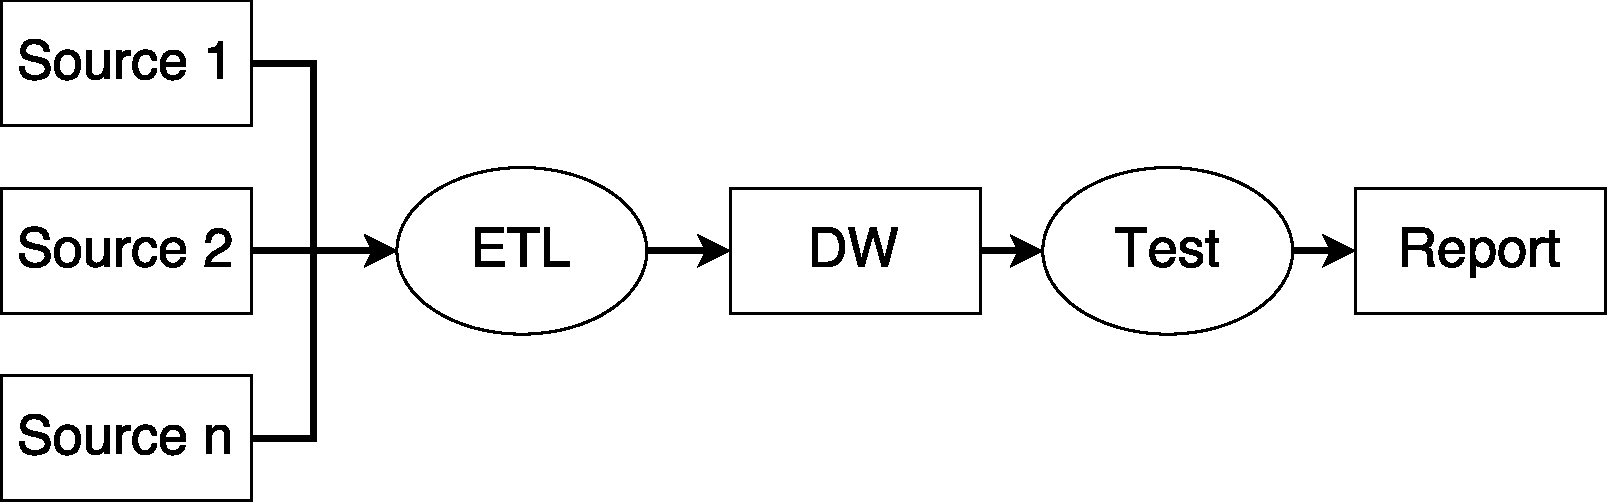
\includegraphics[width=8.5cm]{figures/scenario.pdf}
		\item<3-> Laver DW representation for os
    \item<4-> Udskiftning af sources
			\begin{itemize}
				\item<5-> Tester - Ingen adgang til firmaets sources
				\item<6-> Skrive egne test sources til program
				\item<7-> Ingen grund til at ændre program
			\end{itemize}
  \end{itemize}
\end{frame}

\begin{frame}{DWPopulator begrænsninger}{}
	DWPopulator begrænsninger
  \begin{itemize}
    \item<1-> Kun en DW
    \item<2-> Ingen source eller table objekt instantioner gennem iteration
    \item<3-> Ingen source eller table objekt instantioner gennem imports
  \end{itemize}
\end{frame}

\begin{frame}{DWPopulator begrænsninger}{}
  transform\_visitor.py
	\insertcodefile{CallNode.py}{}
\end{frame}

\begin{frame}{DWPopulator begrænsninger}{}
  DWPopulator begrænsninger
	\begin{itemize}
		\item<1-> Kan ikke udskifte sources på runtime
		\item<2-> Sources erstattes efter position
		\item<3-> Kan ikke erstatte med samme source flere gange
		\item<4-> \insertcodefile{get_id.py}{}
	\end{itemize}
\end{frame}

\subsection{Intermediate Representation}
\begin{frame}{Intermediate Representation}{}
  Hvornår bruges den?
  \begin{itemize}
    \item<1-> Input til predicates
  \end{itemize}
  Hvorfor nyttigt?
  \begin{itemize}
    \item<2-> Giver standart metoder til at tilgå data i skema
		\begin{itemize}
			\item<3-> Table navn giver adgang til specifikt table
			\item<4-> Kan iterere over tables og rækker
			\begin{itemize}
				\item<5-> Subset af kolonner
				\item<6-> Natural joins
			\end{itemize}
		\end{itemize}
  \end{itemize}
\end{frame}

\begin{frame}{Intermediate Representation begrænsninger}{}
  Begrænsinger
  \begin{itemize}
    \item<1-> Facttable må kun have referencer til en snowflake’s root
    \item<2-> Referencer mellem dimensions sker kun i snowflaking
    \item<3->[] 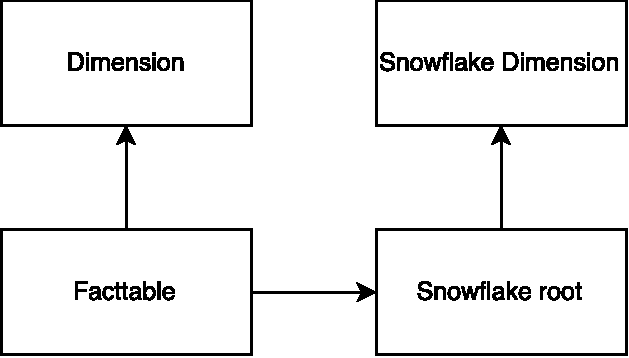
\includegraphics[width=8.5cm]{figures/IRLimitations.pdf}
  \end{itemize}
\end{frame}
